\documentclass{article}

\usepackage{ocencfd}
\usepackage{geometry}
\usepackage{graphicx}
\usepackage{float}
\usepackage{amsfonts}
\usepackage{mathrsfs}
\usepackage{mwe}
\usepackage{subfig}

\title{Introduction to Deep Learning\\Assignment 2} % Sets article title
\author{\textbf{Group 53}\\Chenyu Shi (s3500063); Shupei Li (s3430863); Shuang Fan (s3505847)} % Sets authors name
\documentID{Introduction to Deep Learning Assignment 2} %Should be alphanumeric identifier
\fileInclude{} %Names of file to attach
\date{\today} % Sets date for publication as date compiled
\graphicspath{{fig/}}
\geometry{a4paper, left=2.5cm, right=2.5cm, top=2.5cm, bottom=2.5cm}

% The preamble ends with the command \begin{document}
\begin{document} % All begin commands must be paired with an end command somewhere

\maketitle % creates title using information in preamble (title, author, date)

\section*{Task 1}

\section*{Task 2}
\setcounter{section}{2}
\subsection{Regression}
The regression model structure is shown in Figure \ref{fig:regression}. And its corresponding results are shown in Table \ref{tab:performance}. Because this is a regression task, we use MSE as loss function and Adam as optimizer. This model takes 2207593 trainable parameers, which is relatively high comparing to other models in task2. However, the final common sense loss is still a little bit high, which is 0.7053 hour(about 42.3 minutes). This is mainly caused by the problem of this kind of labels. Representing time in this way doesn't obey common sense. For example, 11:55 will be represented as 11.917 while 0:05 will be represented as 0.0833. Even though in common sense, the difference between 11:55 and 0:05 is only 10 minutes, their reformulated labels 11.917 and 0.0833 have a very high MSE. Therefore, this regression model has a limitted final performance.
\begin{figure}[!h]
	\centering
	\begin{minipage}[t]{0.3\textwidth}%并排放两张图片,每张占页面的0.5,下同。
		\centering
		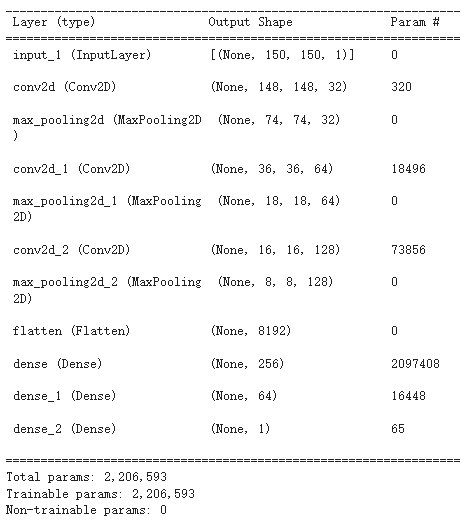
\includegraphics[width=\textwidth]{regression.png}
		\caption{Regression model}
		\label{fig:regression}
	\end{minipage}
	\begin{minipage}[t]{0.3\textwidth}%并排放两张图片,每张占页面的0.5,下同。
		\centering
		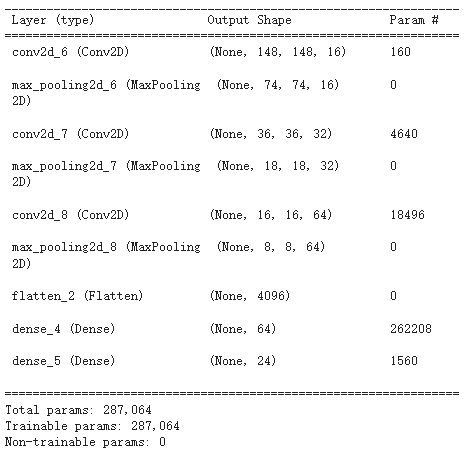
\includegraphics[width=\textwidth]{classification.png}
		\caption{Classification model}
		\label{fig:classification}
	\end{minipage}
	\begin{minipage}[t]{0.3\textwidth}%并排放两张图片,每张占页面的0.5,下同。
		\centering
		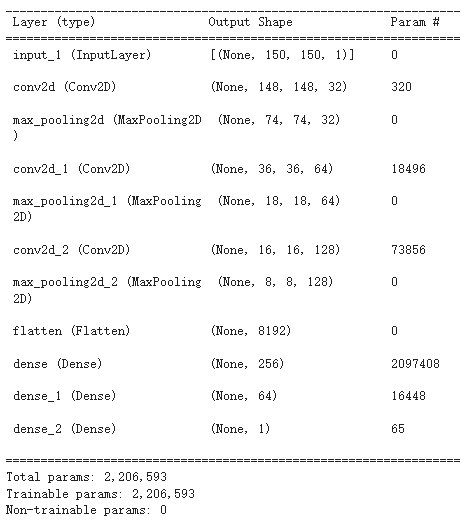
\includegraphics[width=\textwidth]{regression.png}
		\caption{Multi-head model}
		\label{fig:multi-head}
	\end{minipage}
\end{figure}
    \begin{table}[!ht]
	\caption{Results and Algorithm Comparison}
	\label{tab:performance}
	\centering
	\begin{tabular}{cc}
		\toprule
		\textbf{Model} & \textbf{Common Sense Loss(hours)} \\
		\midrule
		Regression & 0.7053 \\
		Classification(24 classes) & 0.6206 \\
		Classification(72 classes) & 0.9517 \\
		Classification(720 classes) & 3.0309 \\
		Multi-head & 0.8634 \\
		\bottomrule
	\end{tabular}
\end{table}
\subsection{Classification}
The regression model structure is shown in Figure \ref{fig:classification}. And its corresponding results are shown in Table \ref{tab:performance}. Thereinto, model structures of 24 classes, 72 classes and 720 classes are only different in last output layers. Because this is a multi-class classification task, we use cross entropy as loss function adn Adam as optimizer. And we can see, although classification model uses much fewer trainable parameters, the final result for 24 classes is better than regression model with a performance of 0.6206 hours(about 37.2 minutes). However, when we increase the number of categories, the performance of model become poorer. And the model of 720 classes even didn't coverge and has a very high common sense loss. That's because this kind of label representation also has its problems. The first problem is that this label representation cannot measure "how much difference two categories have". For example, in 24 classes model, 0:01 and 0:31 are in different categories, and 0:01 and 6:00 are also in different categories. Although the common sense loss between 0:01 and 6:00 are much larger than that between 0:01 and 0:31, the cross entropy loss function in classfication task will give them same loss values. The second big problem is that it's hard for us to balance  sampling interval and samples number. If we have large sampling interval along with a large samples number, the model can get well trained because there are sufficient training data in each class, but the common sense loss within each class becomes rather high. For example, in 24 classes model, 0:01 and 0:29 will be classified into same class even they are almost half an hour apart. On the contrary, if we have small sampling interval along with a small samples number, the common sense loss within each class becomes rather small, but the model itself cannot be well trained due to lack of training data for each class. For example, in 720 classes model, each class will only have 25 pictures for training, validation and test set. That's not a sufficient number for training CNN in a regular way.


\section*{Task 3}
\setcounter{section}{3}
\subsection{Datasets}
We use two datasets in Task 3. Firstly, we explore the performance of different model architectures and the effects of different parameters with MNIST data. After that, we leverage the power of generative models on Butterfly \& Moths data. \par
We directly call Tensorflow API to download the MNIST dataset. However, the original dataset is also available on \url{https://deepai.org/dataset/mnist}. MNIST dataset contains 70,000 grayscale images (28 $\times$ 28 $\times$ 1), whose content is handwritten numbers. \par
Butterfly \& Moths is an open source dataset on Kaggle. There are 13,639 RGB images (224 $\times$ 224 $\times$ 3) composed of 100 butterfly or moth species. Link of the dataset is \url{https://www.kaggle.com/datasets/gpiosenka/butterfly-images40-species?resource=download}.

\subsection{Experimental Set-up}
All experiments are deployed on two servers. Server 1
\subsubsection{MNIST}
We modify the 

\subsection{Results}

\subsection{Discussion: Model Comparison}

\section*{Contributions}
\end{document}
